\section{Erster Commit}
\begin{lstlisting}
$ git status
On branch master

No commits yet

Changes to be committed:
  (use "git rm --cached <file>..." to unstage)
	new file:   Bibliothek.bib
	new file:   Bilder/Versioncontrol.png
	new file:   Bilder/git_Commit.png
	new file:   Commit.tex
	new file:   Einleitung.tex
	new file:   Title.tex
	new file:   initialisierung.tex
	new file:   main.tex

\end{lstlisting}
Um den aktuellen Status zu protokollieren muss der Befehl \inline{git commit} genutzt werden. Dabei werden alle Änderungen an allen Dateien protokolliert, die sich im Status \qq{staged} befinden.

Ist eine Datei neu (war vorher also im Status \qq{untracked} wird dabei eine Kopie der Datei zwischengespeichert. Ist die Datei nur verändert wurden (war vorher somit im Status \qq{modified}) wird nur die Änderung gespeichert.

Ein Commit besteht aus drei Teilen: Einem \qq{parent} Commit - der Commit, der den Status vor den Änderungen angibt -, einer Liste an Änderungen und einer Commit-message. Commit-messages sollten möglichst einheitlich und übersichtlich gestaltet werden. Für Programmcodes gibt \cite{conv-Commit} eine gute Zusammenfassung, wie Commit-messages strukturiert werden können\footnote{In dem Beispiel git zu diesem Bericht wird davon jedoch nicht vollständig Gebrauch gemacht, da es für Latex Dokumente nicht geeignet ist.}.

Wenn der Befehl \inline{git commit} ohne Optionen ausgeführt wird öffnet sich daher automatisch der standard editor (der über \inline{git config --local core.editor} definiert wurde). In diesem Befindet sich eine auskommentierte Übersicht des Commits. Darunter muss eine Commit-Message eingefügt werden. Wir der Editor geschlossen ohne unkommentierten Inhalt hinzugefügt zu haben bricht der Commit ab.
\begin{figure}[!h]
        \centering
        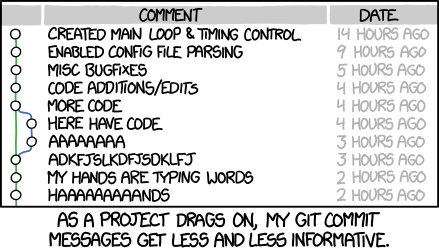
\includegraphics[width=0.5\textwidth]{Bilder/git_commit.png}
        \caption{Eine Commit-tree-Darstellung von XKCD \cite{Munroe}. Die Commit-Messages starten oben mit den ersten Commits sehr vorbildlich. Nach einigen Commits ist zu sehen, dass die Messages keine informationen über den Commit Inhalt mehr haben. Dies ist ein häufiges Problem, wenn zu selten Committed wird kann es schnell passieren, dass nicht mehr klar ist, was sich seit dem letzten Commit alles geändert hat. Dadurch werden Commit-Messages schnell schwer zu schreiben und vernachlässigt.}
        \label{fig:Commit-XKCD}
\end{figure}

In Abb. \ref{fig:Commit-XKCD} ist ein sogenannter \qq{Commit-tree} dargestellt. In einem Commit-tree werden alle existierenden Commits aufgelistet und parent und child Commit miteinander verbunden. Neben jedem Commit wird der jeweilige Commit-header angezeigt. Solch ein Commit-tree sollte eine gute Übersicht über den Verlauf der Entwicklung eines Programms geben. Daher müssen Commit-header möglichst eindeutig und einheitlich verfasst werden.

In Abb. \ref{fig:Commit-XKCD} sieht man jedoch, dass es zunehmend schwerer werden kann zu einem Commit eine gute Beschreibung zu finden. Wenn z.B. viele Änderungen in einem Commit zusammengefasst werden kann es schwer sein einen geeigneten Commit-header zu finden.

Nachdem ein Commit erfolgt ist befinden sich alle Dateien, die vorher im staging Status waren im unmodified Status (siehe Abb. \ref{fig:lifecycle}). 
\begin{lstlisting}
$ git status
On branch master
nothing to commit, working tree clean
\end{lstlisting}
